\documentclass[10pt]{beamer}
%\documentclass[handout, 10pt]{beamer} %aurait supprim� les ``overlays''
\usefonttheme[onlymath]{serif}
\usetheme{Pittsburgh}% le th�me choisi pour ma pr�sentation
%\useoutertheme{smoothbars}
%\useinnertheme{rounded}
\usepackage[french]{babel}
\usepackage[latin1]{inputenc}
\usepackage{amsmath}
\usepackage{amssymb}
\usepackage{geometry}
\usepackage{graphicx}%pour les includegraphics
\usepackage{array}% pour des tableaux particuliers. N�cessaire pour les r�v�ler colonne par colonne
\usepackage{pstricks}
\usepackage{epsfig}
%\usepackage{pst-plot}
\usepackage{ragged2e}

\usepackage{eurosym}

\setbeamertemplate{navigation symbols}{}

\justifying



%\setbeamertemplate{navigation symbols}{}
\setbeamertemplate{footline}
{
  \leavevmode%
  \hbox{%
      \begin{beamercolorbox}[wd=.333333\paperwidth,ht=2.25ex,dp=1ex,center]{author in head/foot}%
        \usebeamerfont{author in head/foot} J�r�me Dugast
      \end{beamercolorbox}%
      \begin{beamercolorbox}[wd=.333333\paperwidth,ht=2.25ex,dp=1ex,center]{title in head/foot}%
        \usebeamerfont{title in head/foot} Microeconomics for Finance - Exchange Economy
      \end{beamercolorbox}%
      \begin{beamercolorbox}[wd=.333333\paperwidth,ht=2.25ex,dp=1ex,right]{date in head/foot}%
        \usebeamerfont{date in head/foot}%\insertshortdate{}\hspace*{2em}
        \insertframenumber{} / \inserttotalframenumber\hspace*{2ex} 
      \end{beamercolorbox}%
  }%
}
\justifying

\colorlet{orange}{red!70!yellow}% mes petites couleurs que j'aime bien
\colorlet{mauve}{blue!70!red}
\colorlet{brouge}{red!70!blue}

%\addtobeamertemplate{footline}{\insertframenumber/\inserttotalframenumber}
%pour ajouter un num�ro de page en bas.% une autre solution : \useoutertheme{shadow}
%\usepackage{beamerthemesplit}

\title{\black {\huge \textbf{Microeconomics for Finance}} \\ \vspace{0.5cm} Equilibrium in an Exchange Economy}

\institute[shortinst]{
\includegraphics[scale=0.15]{Figures/CMJN} }
\author[shortname]{ \bf J�r�me Dugast}

\date{}


\begin{document}


\newtheorem{equi}{Equilibrium}[section]
\newtheorem{ass}{Assumption}
\newtheorem{prop}{Proposition}[section]
\newtheorem{lem}{Lemma}
\newtheorem{cor}{Corollary}
\newtheorem{defi}{Definition}



\renewcommand{\raggedright}{\leftskip=0pt \rightskip=0pt plus 0cm}

\frame{\titlepage}



%\frame{
%\frametitle{Outline}
%\tableofcontents
%}







\frame{
\frametitle{Introduction}


\begin{itemize}
\item An exchange economy corresponds to a situation in which several agents are initially endowed with consumption goods.
\item From a given basket of goods, an agent draws a certain level of ``satisfaction" or \textbf{utility} which is measured by a utility function.
\item Agents are allowed to trade their initial endowments with each other, in a \textbf{Walrasian market}, to possibly increase their utility.
\item The efficiency of the market outcome can be assessed with the concept of \textbf{Pareto optimality}.
\item[]
\item  In this class we focus the simplest setup: 2 agents and 2 goods.
\end{itemize}




}










\frame{
\frametitle{$2\times 2$ Economy}


\begin{itemize}
\item Two agents, $A$ and $B$, and two goods, $1$ and $2$.
%\item[]
\item Initial endowments: 
\item[-] $A$ endowed with quantities $\omega_1^A$ of good $1$, and  $\omega_2^A$ of good $2$
\item[-] $B$ endowed with quantities $\omega_1^B$ of good $1$, and  $\omega_2^B$ of good $2$
\item[]
\item Aggregate resources of goods $1$ and $2$: $\omega_1 = \omega_1^A + \omega_1^B$, $\omega_2 = \omega_2^A + \omega_2^B$.
\item[]
\item Feasible baskets for $A$: $(x_1,x_2)$ with $x_1 \geq 0, x_2 \geq 0$. 
\item Feasible baskets for $B$: $(y_1,y_2)$ with $y_1 \geq 0, y_2 \geq 0$.
\item[]
\item Feasible allocation: a pair of baskets, $\{(x_1,x_2),(y_1,y_2)\}$, such that 
$$x_1+ y_1 = \omega_1, \ \mbox{and} \ x_2+ y_2 = \omega_2$$
\item The \textbf{Edgeworth box} represents feasible allocations.
\end{itemize}



}



\frame{
\frametitle{Edgeworth box}

%\begin{center}
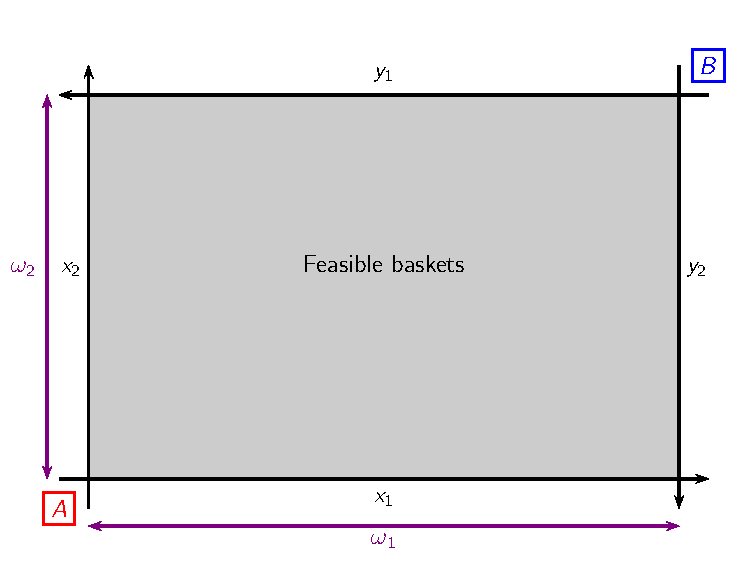
\includegraphics[scale=0.85]{Figures/EdgeworthBox_1}
%\end{center}


}



\frame{
\frametitle{Walrasian Market}

\begin{itemize}
\item Good $1$ can be traded (bought and sold) at price $p_1$.  Good $2$ can be traded at price $p_2$.
\item[]
\item These prices are \underline{not} parameters. Our objectives is determines the prices that clear the markets (s.t demand = supply)
\item[] 
\item Given $p_1$ and $p_2$, $A$'s initial wealth is $W_A= p_1 \omega_1^A + p_2 \omega_2^A$. 
\item[]
\item Feasible baskets under budget constraints for $A$: $(x_1,x_2)$ such that 
$$p_1 x_1 + p_2 x_2 \leq  W_A$$
Optimally her budget is exhausted. She will pick an allocation on the \emph{budget line}: $p_1 x_1 + p_2 x_2 = W_A$. Idem for $B$.
\item[]
\item Budget constraints partition the Edgeworth box.
\end{itemize}


}


\frame{
\frametitle{Bugdet Constraints}

%\textbf{Example:} $p_2=1, \ p_1 =1.5$.

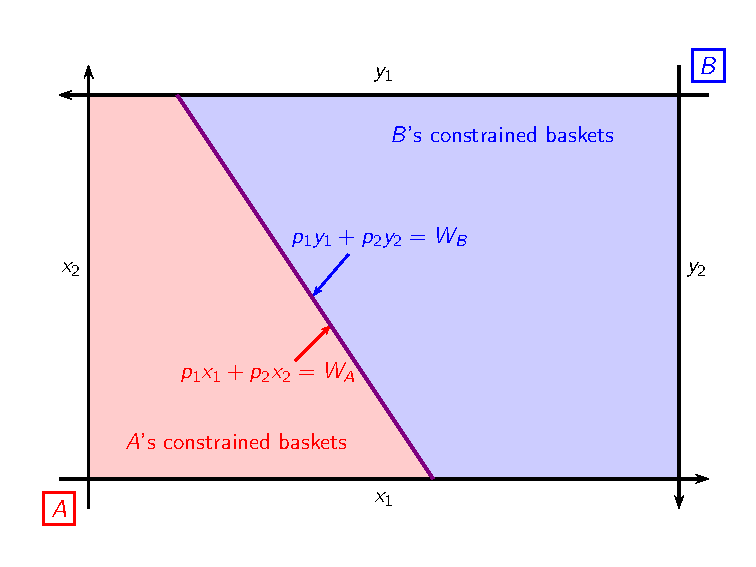
\includegraphics[scale=0.85]{Figures/EdgeworthBox_2}


}



\frame{
\frametitle{Bugdet Constraints}

%\textbf{Example:} $p_2=1, \ p_1 =1.5$.

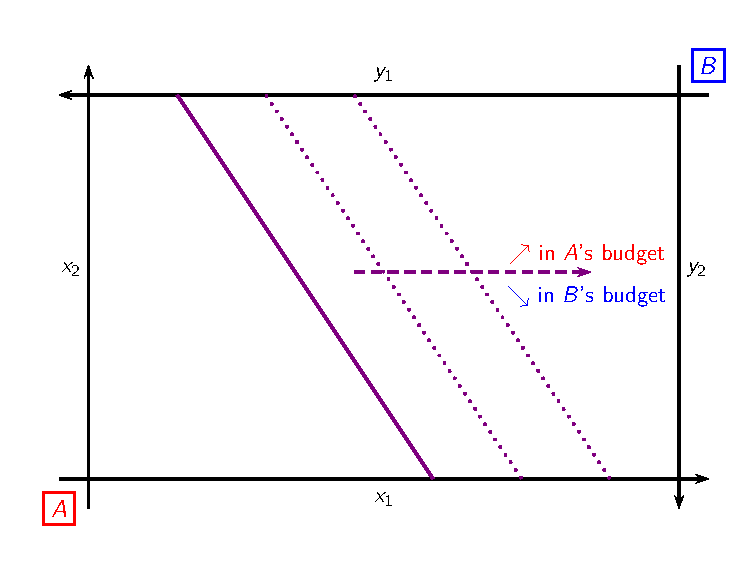
\includegraphics[scale=0.85]{Figures/EdgeworthBox_3}


}



\frame{
\frametitle{Preferences}

\begin{itemize}
\item Individual preferences of $A$ over baskets represented by the utility function, $u^A$. A specific (feasible) basket $(x_1,x_2)$ yields a utility level $u^A(x_1,x_2) \in \mathbb{R}$. Idem for $B$.
\item[]
\item The utility function should be strictly concave, and strictly increasing in each good, that is
$$\frac{\partial u^A}{\partial x_1} > 0, \  \frac{\partial u^A}{\partial x_2} > 0, \ \frac{\partial^2 u^A}{\partial x_1^2} < 0, \  \frac{\partial^2 u^A}{\partial x_2^2} < 0.$$

\item Example: Cobb-Douglas utility function
$$u^A(x_1,x_2) = x_1^{\alpha}x_2^{1-\alpha}, \ \ u^B(y_1,y_2) = y_1^{\beta}y_2^{1-\beta},$$
with $\alpha \in [0,1], \ \beta \in [0,1]$.
\item One can represent iso-utility curves, that sets of baskets generating a given utility level, in the Edgeworth box
\end{itemize}


}



\frame{
\frametitle{Iso-utility Curves}

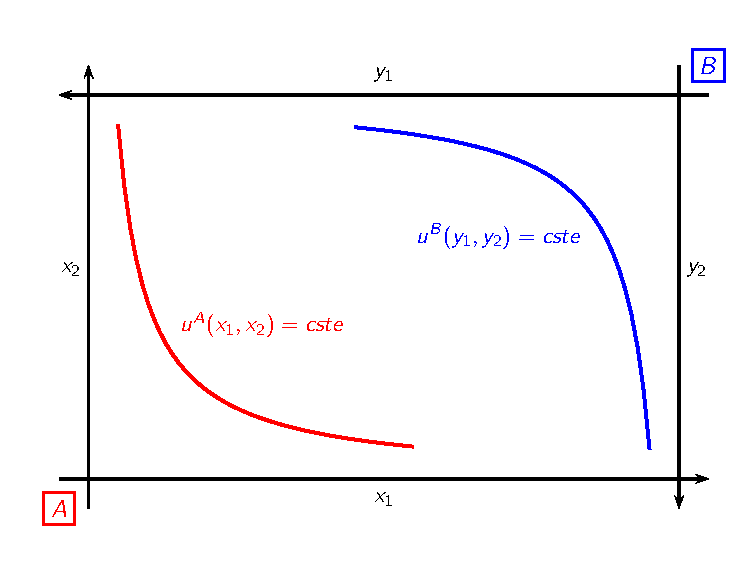
\includegraphics[scale=0.85]{Figures/EdgeworthBox_4}


}



\frame{
\frametitle{Iso-utility Curves}

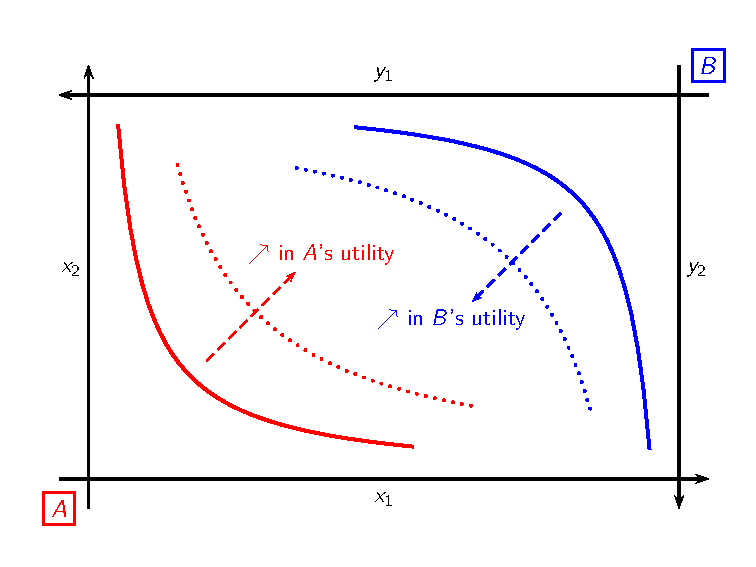
\includegraphics[scale=0.85]{Figures/EdgeworthBox_5}


}





\frame{
\frametitle{Pareto Optimality}


\begin{itemize}
\item Allocation $\{(x_1,x_2),(y_1,y_2)\}$ dominates allocation $\{(x'_1,x'_2),(y'_1,y'_2)\}$ in the Pareto sense if
$$u^A(x_1,x_2) \geq u^A(x'_1,x'_2), \ \mbox{and} \ u^B(y_1,y_2) \geq u^B(y'_1,y'_2),$$
$$\mbox{with at least one strict inequality,}$$
that is if both agent are better off with the first allocation.
\item[]
\item A feasible allocation $\{(x_1,x_2),(y_1,y_2)\}$ is \emph{Pareto optimal} if it is not dominated by any feasible allocation in the Pareto sense. 

Put differently, any other feasible allocation would make (at least) one agent worse off.
\item[]
\item Typically, there are multiple (a set of) Pareto optimal allocations.
\end{itemize}



}


\frame{
\frametitle{Pareto Optimality}

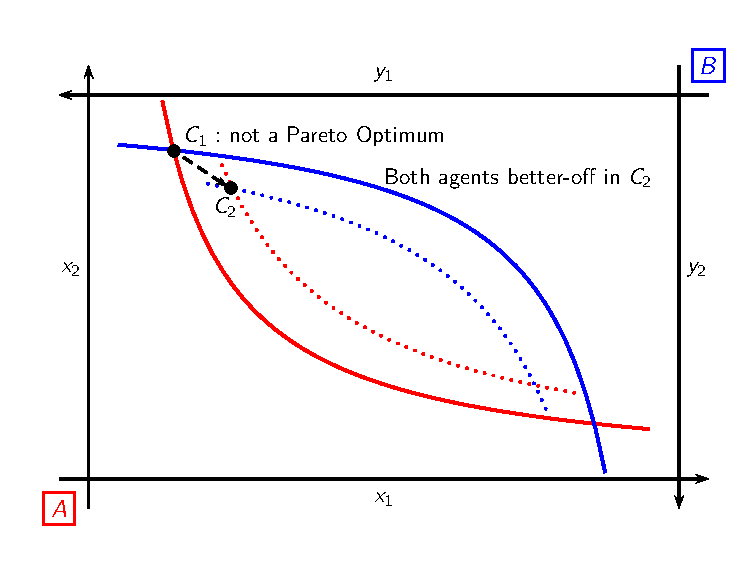
\includegraphics[scale=0.85]{Figures/EdgeworthBox_6}


}


\frame{
\frametitle{Pareto Optimality}

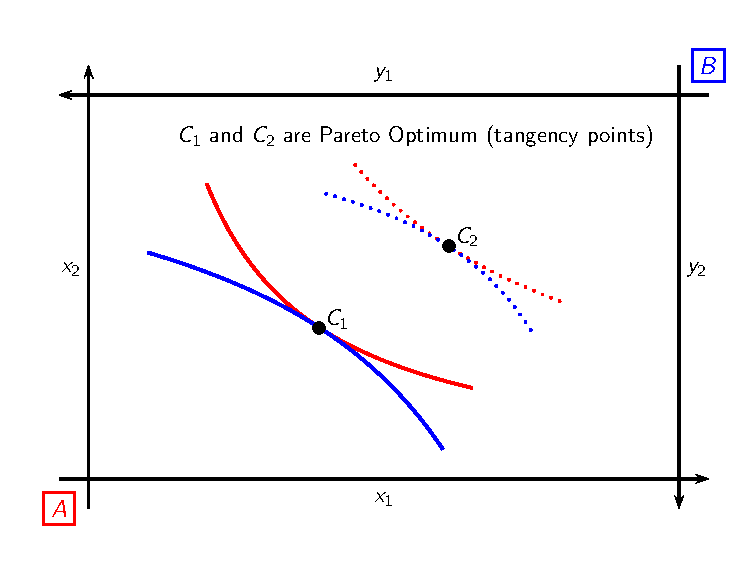
\includegraphics[scale=0.85]{Figures/EdgeworthBox_7}


}


\frame{
\frametitle{Individual Optimization}

\begin{itemize}
\item \textbf{Result:} Under the strict concavity and increasing assumptions on $u^A$, and for given prices $p_1$ and $p_2$, there exists a unique \emph{optimal} basket $(x_1,x_2)$. It maximizes $u^A(x_1,x_2)$ under the budget constraint.
\item[]
\item Based on this existence and uniqueness result, one can define the demand function of $A$.
\item[$\rightarrow$] The demand function of $A$ maps each set of price $(p_1,p_2)$ to the optimal basket, $(x_1(p_1,p_2),x_2(p_1,p_2))$.
\item[]
\item Idem for $B$.
\end{itemize}


}



\frame{
\frametitle{Individual Optimization}

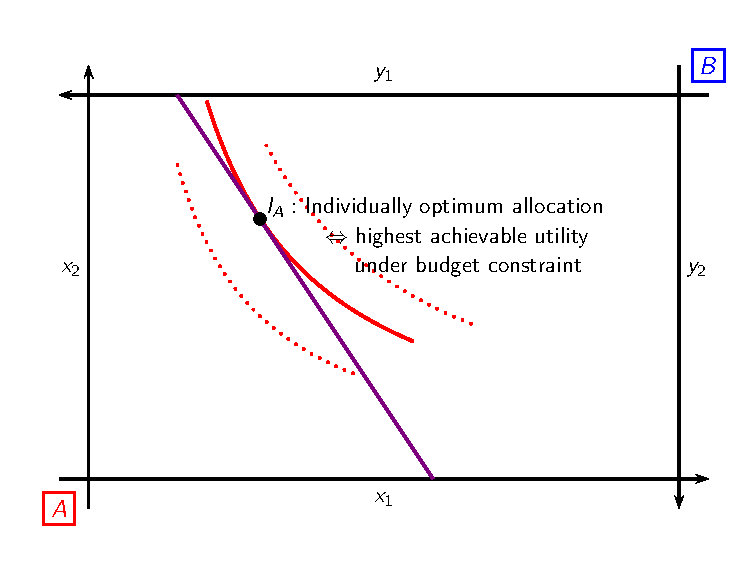
\includegraphics[scale=0.85]{Figures/EdgeworthBox_8}

}





\frame{
\frametitle{Individual Optimization}

\begin{itemize}
\item The constrained optimization program of $A$ can be written as:
$$\max_{x_1,x_2} u^A(x_1,x_2) \ \ \mbox{under constraint (u.c)} \ \ p_1 x_1 + p_2 x_2 = p_1 \omega_1^A + p_2 \omega_2^A$$
\item In the $2 \times 2$ economy, this multi-dimensional optimization problem can be turned into a one-dimensional one. Use the budget constraint to define $x_2$ as a function of $x_1$:
$$x_2 = \frac{p_1}{p_2}\omega_1^A +  \omega_2^A - \frac{p_1}{p_2}x_1.$$
\item The optimization program becomes
$$\max_{x_1} u^A\left(x_1,\frac{p_1}{p_2}\omega_1^A +  \omega_2^A - \frac{p_1}{p_2}x_1\right)$$
\item It is solved by taking the \emph{first order condition (F.O.C)},
$$\frac{\partial}{\partial x_1} \left\{u^A\left(x_1,\frac{p_1}{p_2}\omega_1^A +  \omega_2^A - \frac{p_1}{p_2}x_1\right) \right\} = 0,$$
to obtain directly the optimal $x_1(p_1,p_2)$, and then $x_2(p_1,p_2)$. 
\end{itemize}


}


\frame{
\frametitle{Individual Optimization}

\begin{itemize}
\item The standard optimization technique is the \textbf{Lagrangian method}.
\item One defines the Lagrangian of the constrained optimization program:
$$\mathcal{L}^A =  u^A(x_1,x_2) + \lambda^A (p_1 \omega_1^A + p_2 \omega_2^A - p_1 x_1 - p_2 x_2)$$
where $\lambda^A$ is a new variable called the \emph{Lagrange multiplier}.
\item The Lagrangian (and its multiplier) is specific to $A$. $B$ has his own.
\item[]
\item It is solved by taking three F.O.C's,
$$\frac{\partial \mathcal{L}^A }{\partial x_1}= 0, \ \frac{\partial \mathcal{L}^A }{\partial x_2}= 0, \ \mbox{and} \ \frac{\partial \mathcal{L}^A }{\partial \lambda^A}= 0$$
(the last one returns the budget constraint).
\end{itemize}


}






\frame{
\frametitle{Individual Optimization}

\begin{itemize}
\item Taking the two first F.O.C's of the Lagrangian yields
$$\frac{\partial u^A }{\partial x_1}= \lambda^A p_1, \ \mbox{and} \ \frac{\partial u^A }{\partial x_2}= \lambda^A p_2$$
\item Taking the ratio yields:
$$\left.\frac{\partial u^A }{\partial x_1}\right/\frac{\partial u^A }{\partial x_2} = \frac{p_1}{p_2}$$
That is a \textit{``slope of the iso-utility curve = slope of the budget line"} condition.
\item[]
\item As the optimal allocation should be on the budget line, it is uniquely pinned-down as the tangency  point between an iso-utility curve and the budget line. 
\end{itemize}


}




\frame{
\frametitle{Individual Optimization}

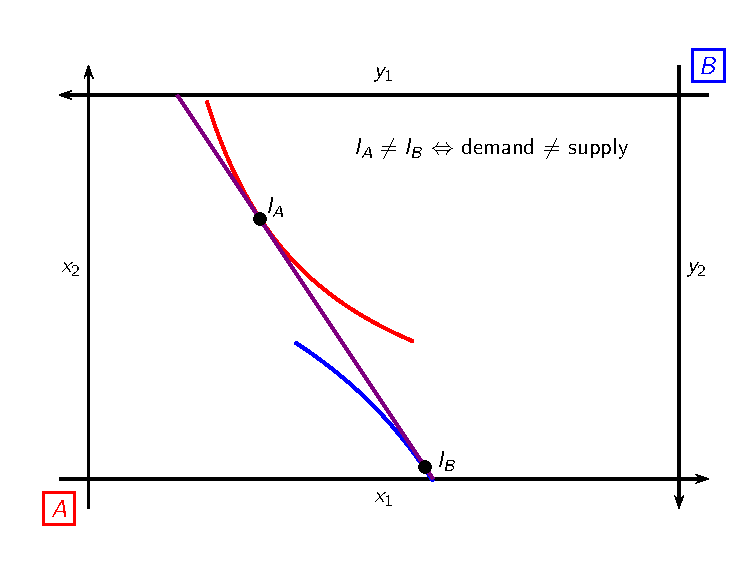
\includegraphics[scale=0.85]{Figures/EdgeworthBox_9}

}




\frame{
\frametitle{Walrasian Equilibrium}

\textbf{Definition.} An (Walrasian) equilibrium is $\{(x^*_1,x^*_2),(y^*_1,y^*_2),p_1^*,p_2^*\}$ such that
\begin{enumerate}
\item $(x^*_1,x^*_2)$ maximizes $u^A(x_1,x_2)$ u.c $p_1^* x_1 + p_2^* x_2 = p_1^* \omega_1^A + p_2^* \omega_2^A$
\item $(y^*_1,y^*_2)$ maximizes $u^B(y_1,y_2)$ u.c $p_1^* y_1 + p_2^* y_2 = p_1^* \omega_1^B + p_2^* \omega_2^B$
\item market clearing: $x^*_1+ y^*_1 = \omega_1$ and $x^*_2+ y^*_2 = \omega_2$
\item[]
\end{enumerate}
Equilibrium prices are not uniquely determined - only up to a scalar $\Rightarrow$ one can choose a numeraire, for instance $p^*_2 = 1$.

\vspace{0.5cm} 

\textbf{First Welfare Theorem.} If $\{(x^*_1,x^*_2),(y^*_1,y^*_2),p_1^*,p_2^*\}$ is an equilibrium then $\{(x^*_1,x^*_2),(y^*_1,y^*_2)\}$ is a Pareto optimal allocation.

}



\frame{
\frametitle{Walrasian Equilibrium}

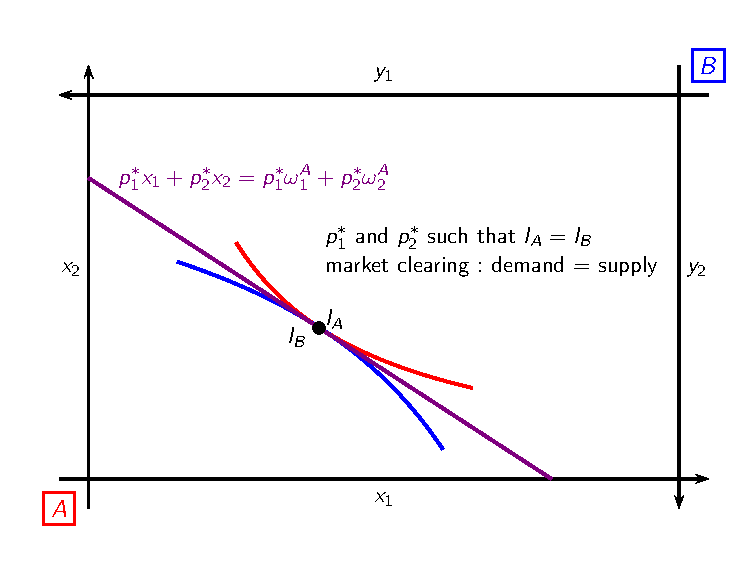
\includegraphics[scale=0.85]{Figures/EdgeworthBox_10}

}




\frame{
\frametitle{Further (Important) Results}

\begin{itemize}
\item \textbf{Second Welfare Theorem.} If $\{(x^*_1,x^*_2),(y^*_1,y^*_2)\}$ is a Pareto optimal allocation, then it is the allocation of an equilibrium with transfers.
\item[]
\item Equilibrium + transfer = take 100\euro \,  from $A$, give it to $B$, and let them trade out of their endowments + transfers.
\item[$\rightarrow$] It means that taxes allow to reach the Pareto optimum we wish among the many.
\item[]
\item All the results can be generalized to an economy with $N \geq 2$ agents and $L\geq 2$ goods.
\end{itemize}

}









\end{document}
